\section{Calculation of the Numenta Anonamly Metric Score}\label{app:numenta-score}
The Numenta Anomaly Metric Score for a single time series is the addition of
\begin{enumerate}[a.)]
    \item the sum of scores for every \defref{def:detection} (given by \cref{eq:score-per-detection}) and 
    \item the score for missed anomaly windows (false negatives) (given by \cref{eq:score-per-fn}).
\end{enumerate}

\begin{align}
    \sigma(t)&= \left(W_{TP} - W_{FP}\right) \left(\frac{1}{1 + e^{5t}}\right) - 1\label{eq:score-per-detection}\\
    \phi(F)&= W_{FN} * \bigl|F\bigr|\label{eq:score-per-fn}\\
    \text{Score}&= \left(\sum_{t\in T}{\sigma(t)}\right) + \phi(F)\label{eq:score-final}
\end{align}
where:
\begin{conditions}
    t &:= & the relative timestamp/position of the detection within the window.\\
    W_{\left\{TP, FP, FN\right\}} &:= & the weights attributed to true and false positives and false negatives respectively.\\
    F &:= & the set of false positives (anomaly windows without any detections).\\
    T &:= & the set of time stamps associated with the detections.
\end{conditions}

The final score per time series is calculated by \cref{eq:score-final}~\cite[cf][]{Lavin.2015}.
An example of the scoring function can be seen in \cref{fig:anomaly-score-example}.

\begin{figure}[htp!]
    \centering
    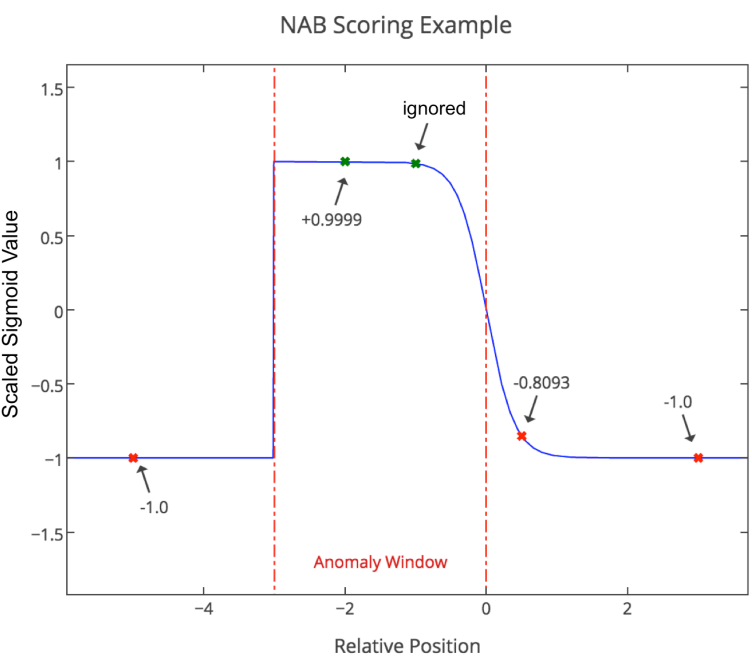
\includegraphics[width=.6\textwidth]{anomaly_scoring.png}
    \caption[Example of anomaly scoring function]{Example application of the anomaly
    scoring function. Illustration adopted from~\cite{Lavin.2015}. The following
    text (blue) is cited from \textcite{Lavin.2015}:
    {\color{blue}
    Scoring example for a sample anomaly window, where the values
    represent the scaled sigmoid function, the second term in \cref{eq:score-per-detection}.
    The first point is an FP preceding the anomaly window (red dashed lines) and
    contributes -1.0 to the score. Within the window we see two detections, and
    only count the earliest TP for the score. There are two FPs after the window.
    The first is less detrimental because it is close to the window, and the second
    yields -1.0 because it’s too far after the window to be associated with the true
    anomaly. TNs make no score contributions. The scaled sigmoid values are
    multiplied by the relevant application profile weight, as shown in Eq.,
    the NAB score for this example would calculate as: 
    \(-1.0W_{FP} + 0.9999W_{TP} - 0.8093W_{FP} - 1.0W_{FP}\).
    With the standard application profile this would result in a total score of
    \(0.6909\).}
    }\label{fig:anomaly-score-example}
\end{figure}\clearpage

\section{Additional Plots of the Datasets}\label{sect:additonal-plots-dataset}
This section provides additional time series plots from \gls{nab}.
% Artificial Data art_daily_flatmiddle  art_daily_jumpsdown art_daily_nojump art_load_balancer_spikes
\begin{figure}[htp!]
    \centering
    \begin{subfigure}[t]{.49\linewidth}
        \centering
        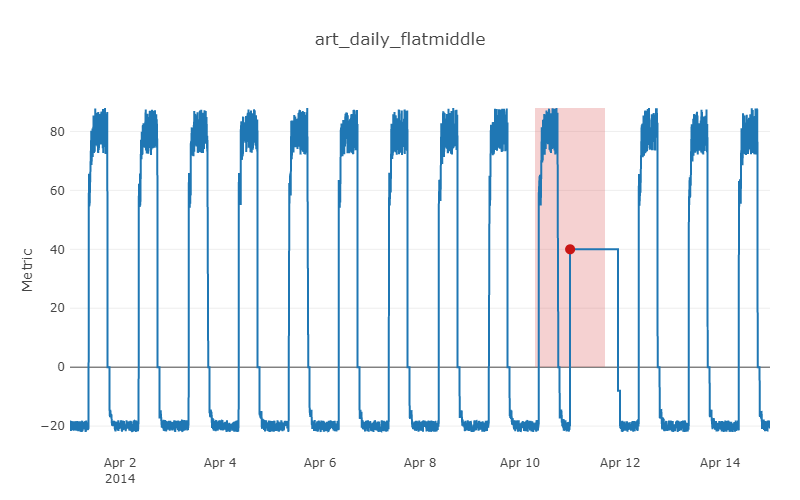
\includegraphics[width=\textwidth]{anomaly_types_examples/final/png/art_daily_flatmiddle.png}
        \subcaption{art\_daily\_flatmiddle.csv}\label{app-fig:art_daily_flatmiddle}
    \end{subfigure}
    \begin{subfigure}[t]{.49\linewidth}
        \centering
        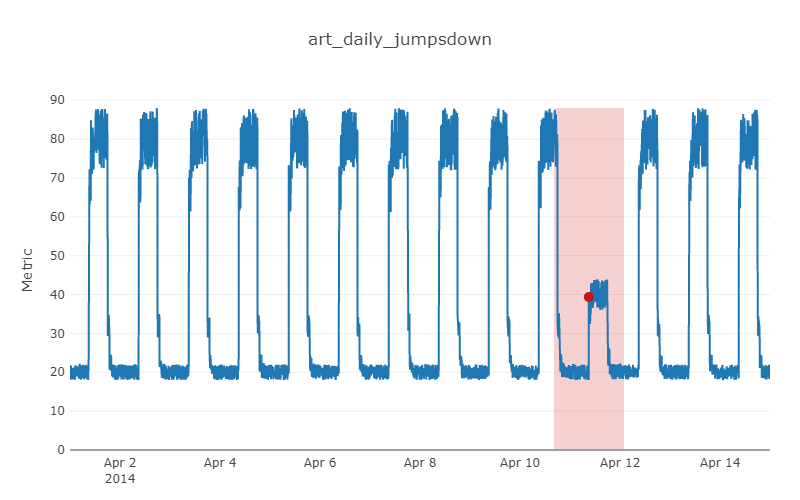
\includegraphics[width=\textwidth]{anomaly_types_examples/final/png/art_daily_jumpsdown.png}
        \subcaption{art\_daily\_jumpsdown.csv}\label{app-fig:art_daily_jumpsdown}
    \end{subfigure}
    \begin{subfigure}[t]{.49\linewidth}
        \centering
        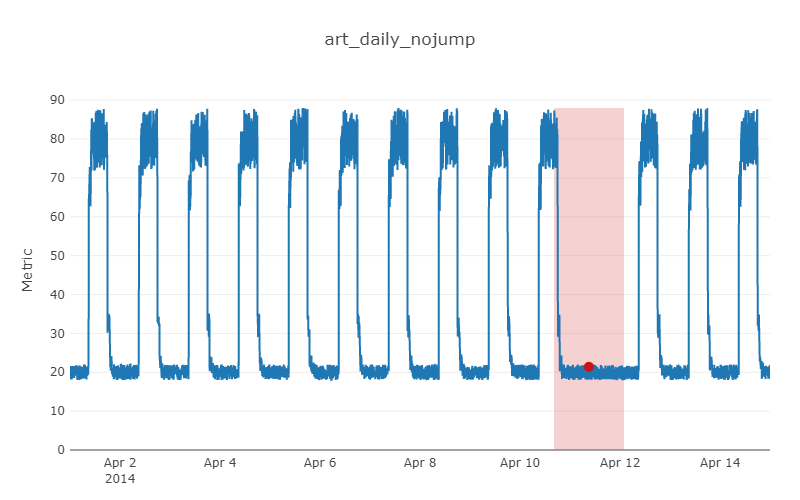
\includegraphics[width=\textwidth]{anomaly_types_examples/final/png/art_daily_nojump.png}
        \subcaption{art\_daily\_nojump.csv}\label{app-fig:art_daily_nojump}
    \end{subfigure}
    \begin{subfigure}[t]{.49\linewidth}
        \centering
        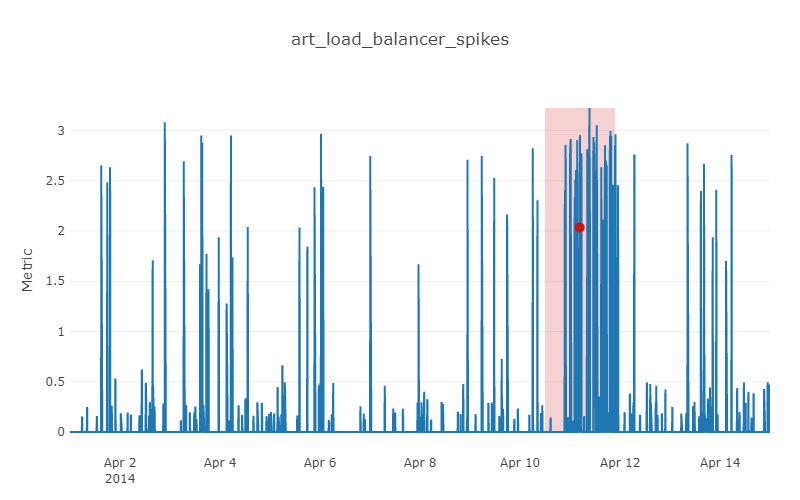
\includegraphics[width=\textwidth]{anomaly_types_examples/final/png/art_load_balancer_spikes.png}
        \subcaption{art\_load\_balancer\_spikes.csv}\label{app-fig:art_load_balancer_spikes}
    \end{subfigure}
    \caption{Artificial anomaly samples}\label{fig:artificial-anomaly-types}
\end{figure}
% Mean: ec2_cpu_utilization_53ea38 grok_asg_anomaly
\begin{figure}[htp!]
    \centering
    \begin{subfigure}[t]{.49\linewidth}
        \centering
        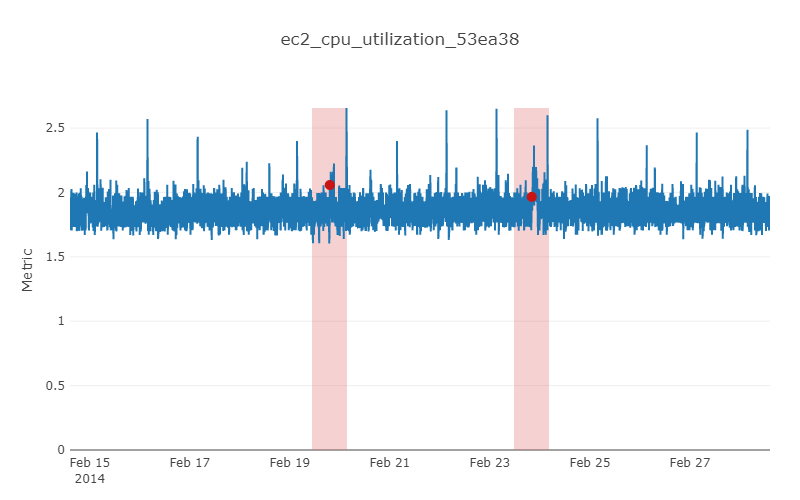
\includegraphics[width=\textwidth]{anomaly_types_examples/final/png/ec2_cpu_utilization_53ea38.png}
        \subcaption{ec2\_cpu\_utilization\_53ea38.csv}\label{app-fig:ec2_cpu_utilization_53ea38}
    \end{subfigure}
    \begin{subfigure}[t]{.49\linewidth}
        \centering
        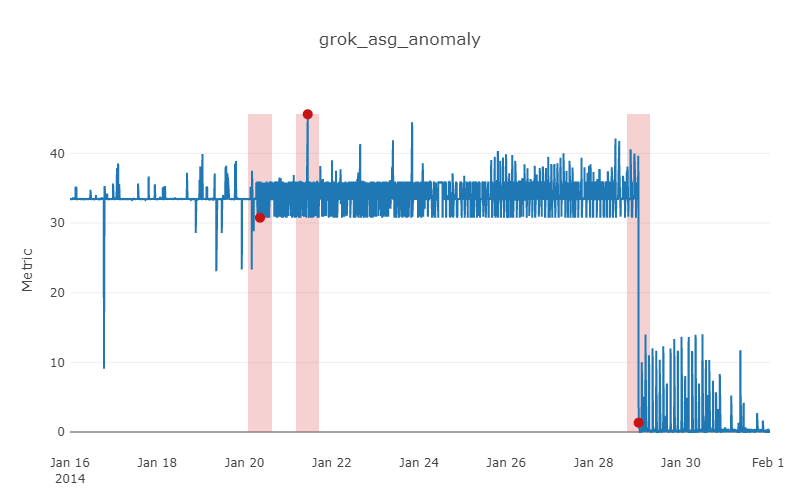
\includegraphics[width=\textwidth]{anomaly_types_examples/final/png/grok_asg_anomaly.png}
        \subcaption{grok\_asg\_anomaly.csv}\label{app-fig:grok_asg_anomaly}
    \end{subfigure}
    \caption{(\subref{app-fig:ec2_cpu_utilization_53ea38}) shows contextual anomalies, (\subref{app-fig:grok_asg_anomaly}) shows two change points and a point-anomaly.}\label{fig:artificial-anomaly-types}
\end{figure}
% Spikes:
% ec2_cpu_utilization_24ae8d ec2_network_in_5abac7 ec2_request_latency_system_failure elb_request_count_8c0756 Twitter_volume_CRM Twitter_volume_CVS Twitter_volume_KO ambient_temperature_system_failure
\begin{figure}[htp!]
    \centering
    \begin{subfigure}[t]{.49\linewidth}
        \centering
        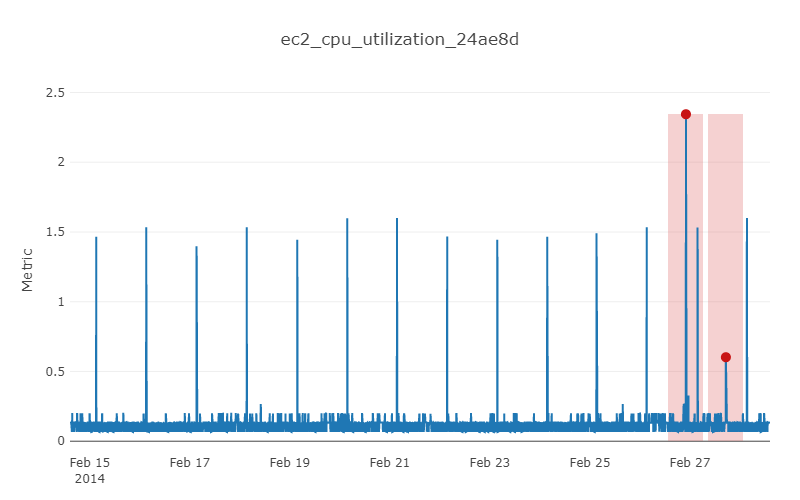
\includegraphics[width=\textwidth]{anomaly_types_examples/final/png/ec2_cpu_utilization_24ae8d.png}
        \subcaption{ec2\_cpu\_utilization\_24ae8d.csv}\label{app-fig:ec2_cpu_utilization_24ae8d}
    \end{subfigure}
    \begin{subfigure}[t]{.49\linewidth}
        \centering
        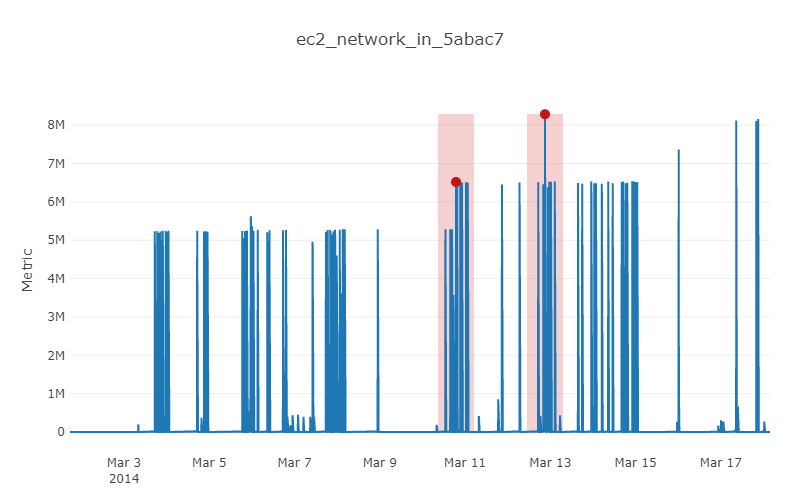
\includegraphics[width=\textwidth]{anomaly_types_examples/final/png/ec2_network_in_5abac7.png}
        \subcaption{ec2\_network\_in\_5abac7.csv}\label{app-fig:ec2_network_in_5abac7}
    \end{subfigure}
    \begin{subfigure}[t]{.49\linewidth}
        \centering
        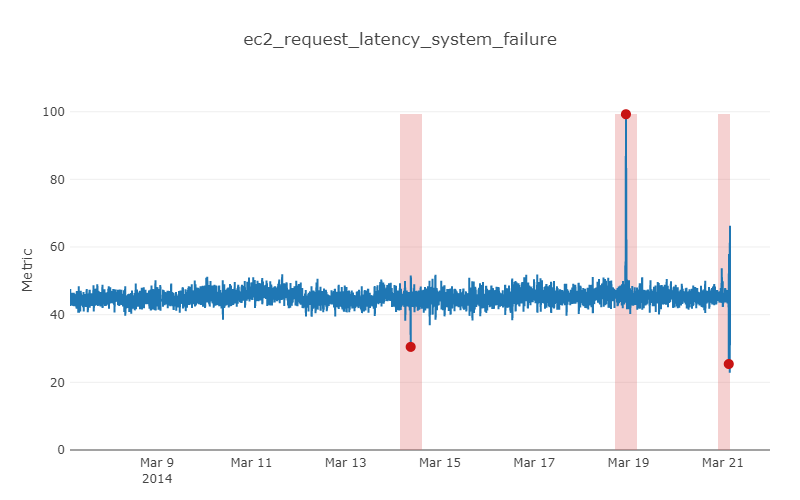
\includegraphics[width=\textwidth]{anomaly_types_examples/final/png/ec2_request_latency_system_failure.png}
        \subcaption{ec2\_request\_latency\_system\_failure.csv}\label{app-fig:ec2_request_latency_system_failure}
    \end{subfigure}
    \begin{subfigure}[t]{.49\linewidth}
        \centering
        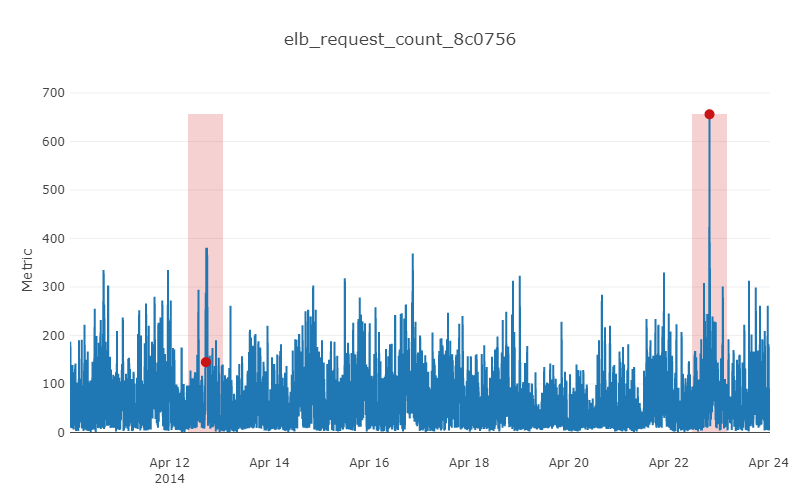
\includegraphics[width=\textwidth]{anomaly_types_examples/final/png/elb_request_count_8c0756.png}
        \subcaption{elb\_request\_count\_8c0756.csv}\label{app-fig:elb_request_count_8c0756}
    \end{subfigure}
    \begin{subfigure}[t]{.49\linewidth}
        \centering
        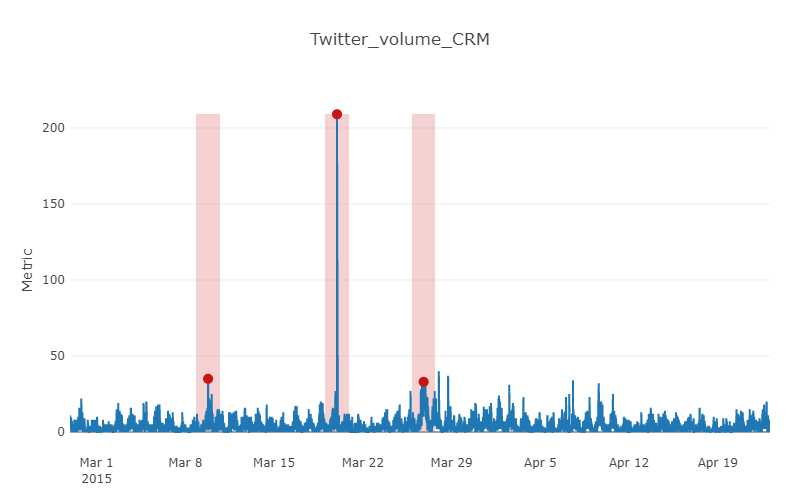
\includegraphics[width=\textwidth]{anomaly_types_examples/final/png/Twitter_volume_CRM.png}
        \subcaption{Twitter\_volume\_CRM.csv}\label{app-fig:Twitter_volume_CRM}
    \end{subfigure}
    \begin{subfigure}[t]{.49\linewidth}
        \centering
        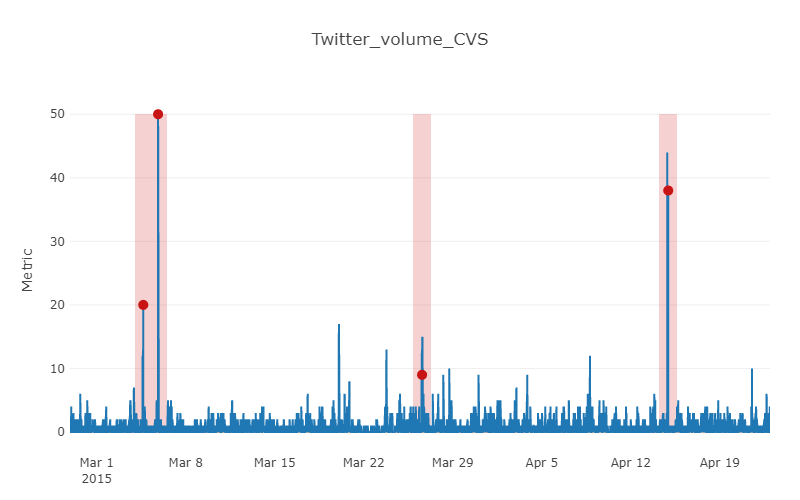
\includegraphics[width=\textwidth]{anomaly_types_examples/final/png/Twitter_volume_CVS.png}
        \subcaption{Twitter\_volume\_CVS.csv}\label{app-fig:Twitter_volume_CVS}
    \end{subfigure}
    \begin{subfigure}[t]{.49\linewidth}
        \centering
        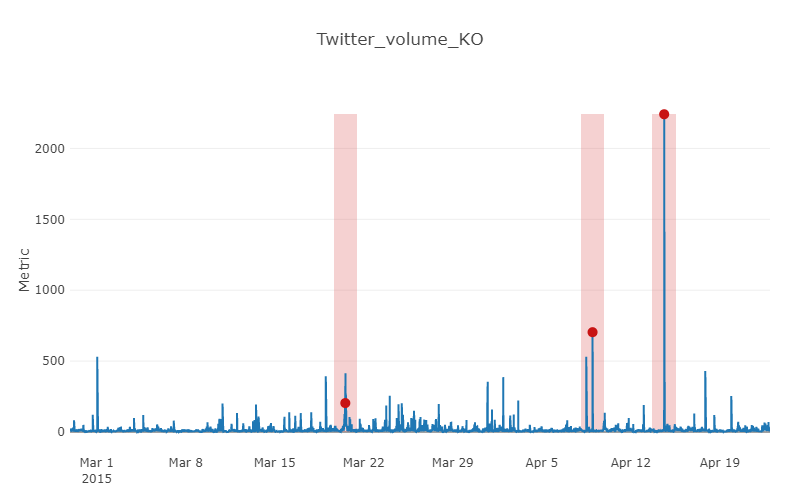
\includegraphics[width=\textwidth]{anomaly_types_examples/final/png/Twitter_volume_KO.png}
        \subcaption{Twitter\_volume\_KO.csv}\label{app-fig:Twitter_volume_KO}
    \end{subfigure}
    \begin{subfigure}[t]{.49\linewidth}
        \centering
        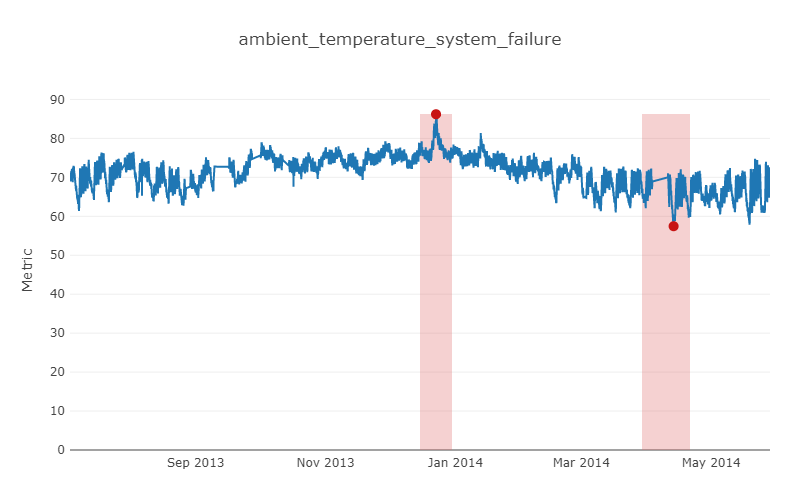
\includegraphics[width=\textwidth]{anomaly_types_examples/final/png/ambient_temperature_system_failure.png}
        \subcaption{ambient\_temperature\_system\_failure.csv}\label{app-fig:ambient_temperature_system_failure}
    \end{subfigure}
    \caption{Point Anomalies. All illustrations by the author.}\label{fig:spiking-types}
\end{figure}\clearpage



\section{Other Datasets}
% Table of several univariate datasets
\begin{table}[h]\centering
    \ra{1.3}
        \begin{tabular}{l}
            Dataset                                                                                                                             \\\midrule
            \href{https://github.com/numenta/NAB}{Numenta Anomaly Benchmark}                                                                    \\\addlinespace
            \href{https://www.kaggle.com/averkij/tennessee-eastman-process-simulation-dataset}{Tennessee Eastman Process Simulation Dataset}    \\\addlinespace
            \href{https://github.com/alan-turing-institute/TCPDBench}{Turing Change Point Benchmark}                                            \\\addlinespace
            \href{https://itrust.sutd.edu.sg/testbeds/secure-water-treatment-swat/}{Secure Water Treatment}                                     \\\addlinespace
            \href{https://en.wikipedia.org/wiki/Makridakis\_Competitions}{M-Competitions}                                                       \\\addlinespace
            \href{https://webscope.sandbox.yahoo.com/catalog.php?datatype=s\&did=70}{Yahoo! Webscope S5}                                        \\
        \end{tabular}
    \caption{Univariate Datasets}\label{tab:univariate-datasets}
\end{table}

% Table of several multivariate datasets
\begin{table}[h]\centering
    \ra{1.3}
        \begin{tabular}{l}
            Dataset                                                                                                                             \\\midrule
            \href{https://www.kaggle.com/anomalydetectionml/features}{Data from: Machine Learning-based Anomaly Detection in Software Systems}  \\\addlinespace
            \href{https://github.com/ricardovvargas/3w_dataset}{3W Dataset}                                                                     \\\addlinespace
            \href{https://www.kaggle.com/rkuo2000/nasa-bearing-sensor-data/notebooks}{NASA Bearing Sensor Data}                                 \\\addlinespace
            \href{https://github.com/chickenbestlover/RNN-Time-series-Anomaly-Detection}{HOT SAX Datasets}                                      \\\addlinespace
            \href{https://github.com/khundman/telemanom}{Soil Moisture Active Passive (SMAP)}                                                   \\\addlinespace
            \href{https://github.com/khundman/telemanom}{Mars Science Laboratory  (MSL)}                                                        \\\addlinespace
            \href{https://www.kaggle.com/icsdataset/hai-security-dataset}{HIL-based Augmented ICS}                                              \\
        \end{tabular}
        \caption{Multivariate-Datasets}\label{tab:multivariate-datasets}
\end{table}\clearpage


\section{Algorithm Selection}\label{sect:algorithms}
% Curation from
\begin{table}[h]\centering
    \ra{1.3}
        \begin{tabular}{l}
            Curated List                                                                                    \\\midrule                                                                               
            \url{https://github.com/cuge1995/awesome-time-series}                                           \\\midrule                                                                               
            \url{https://github.com/xephonhq/awesome-time-series-database}                                  \\\addlinespace
            \url{https://github.com/MaxBenChrist/awesome_time_series_in_python}                             \\\addlinespace
            \url{https://github.com/cuge1995/awesome-time-series}                                           \\\addlinespace
            \url{https://github.com/yzhao062/anomaly-detection-resources#34-time-series-outlier-detection}  \\\addlinespace
            \url{https://github.com/rob-med/awesome-TS-anomaly-detection}                                   \\\addlinespace
            \url{https://www.kaggle.com/general/185462}                                                     \\
        \end{tabular}
    \caption{Curated lists for open source anomaly detection libraries}\label{tab:curation-lists}
\end{table}

% Libraries for anomaly detection
\begin{table}[h]\centering
    \ra{1.3}
    \resizebox{\textwidth}{!}{%
        \begin{tabular}{lllll}
            Library                                                                                                 & Models    & Version   & Latest Commit     & Stars \\\midrule
            \href{https://github.com/arundo/adtk}{Anomaly Detection Toolkit (ADTK)}                                 & \makecell[l]{Statistical Models:\\\tabitem AR\\\tabitem Seasonal Pattern/Decomposition\\\tabitem Generalized ESD-Test\\\tabitem Difference in Mean\\\tabitem Difference in QR/IQR\\\tabitem Difference in Volatility; \\\\ML:\\\tabitem Clustering}                                                                                                                                                                           & 0.6.2     & 17th April 2020   & 582   \\\addlinespace
            \href{https://github.com/smirmik/CAD}{Contextual Anomaly Detector}                                      & No Documentation. Winner of NAB 2016                                                                                                                                                                                                                                                                                                                                                                                          & /         & 10th August 2016  & 63    \\\addlinespace
            \href{https://github.com/MentatInnovations/datastream.io}{datastream.io}                                & \makecell[l]{Focused on integration into ELK-stack;\\ Gaussian-Distribution and Difference in Percentile}                                                                                                                                                                                                                                                                                                                     & /         & 20th Feb 2018     & 804   \\\addlinespace 
            \href{https://github.com/NetManAIOps/donut}{DONUT}                                                      & Variational Auto-Encoder~\cite{Xu.2018}                                                                                                                                                                                                                                                                                                                                                                                       & /         & 6th March         & 298   \\\addlinespace 
            \href{https://github.com/hastic}{hastic}                                                                & \makecell[l]{Focused on Grafana.\\Thresholding on seasonality adjusted and exponentially smoothed data.}                                                                                                                                                                                                                                                                                                                      & /         & 26th Dec 2020     & 274   \\\addlinespace 
            \href{https://github.com/linkedin/luminol}{luminol}                                                     & Bitmap-Transformation~\cite{Wei.2005}, Single Exponential Smoothing;                                                                                                                                                                                                                                                                                                                                                          & 0.4       & 9th Jan 2018      & 861   \\\addlinespace 
            \href{https://github.com/datamllab/pyodds}{PyODDS} / \href{https://github.com/yzhao062/pyod}{PyOD}      & \makecell[l]{Statistical Models:\\\tabitem Local Outlier Factor\\\tabitem Clustering Based Local Outlier Factor\\\tabitem Histogram-Based Outlier Score\\\tabitem Isolation Forest\\\tabitem kNN\\\tabitem One-Class SVM\\\tabitem PCA\\\tabitem Robust Covariance\\\tabitem Subspace Outlier Detection\\\tabitem Luminol\\ Deep Learning:\\\tabitem LSTMAD\cite{Malhotra.2015}\\\tabitem DAGMM~\cite{Zong.2018}}             & /         & 8th May 2020      & 132   \\\addlinespace 
            \href{https://github.com/kLabUM/rrcf}{rrcf}                                                             & Robust Random Cut Forest~\cite{Guha.2016}                                                                                                                                                                                                                                                                                                                                                                                     & 0.4.3     & 10th June 2020    & 271   \\\addlinespace 
            \href{https://github.com/chickenbestlover/RNN-Time-series-Anomaly-Detection}{rnn ts anomaly detection}  & LSTM, GRU, SRU                                                                                                                                                                                                                                                                                                                                                                                                                & /         & 21st Oct 2020     & 684   \\\addlinespace 
            \href{https://github.com/datamllab/tods}{TODS: Time-series Outlier Detection System}                    & DeepLog~\cite{Du.2017}, Telemanom Matrix Profile, PyOD algorithms                                                                                                                                                                                                                                                                                                                                                             & /         & 5th Jan 2021      & 258   \\\addlinespace
            \href{https://github.com/earthgecko/skyline}{Skyline}                                                   & Ensemble of statistical tests like Kolmogorov-Smirnov, Grubbs, deviation from median\ldots                                                                                                                                                                                                                                                                                                                                    & 2.0       & 22th Dec 2020     & 284   \\\addlinespace
            \href{https://github.com/tsurubee/banpei}{Banpei}                                                       & Hotelling's theory~\cite{Hotelling.1990} and Singular Spectrum Transformation                                                                                                                                                                                                                                                                                                                                                 & /         & 21st Sept 2020    & 222   \\\addlinespace
            \href{https://github.com/numenta/nupic}{NuPIC}                                                          & Numenta HTM                                                                                                                                                                                                                                                                                                                                                                                                                   & /         & 23 Oct 2019       & 6.2k   \\\addlinespace
            \href{https://github.com/matrix-profile-foundation/matrixprofile}{MPF}                                  & Matrix Profile                                                                                                                                                                                                                                                                                                                                                                                                                & /         & 26th Dec 2020     & 121    \\
        \end{tabular}
    }
    \caption{Boundary Focused Detection Libraries, accessed last: 8th Jan 2021}\label{tab:ad-packages}
\end{table}


% Libraries for forecasting
\begin{table}[h]\centering
    \ra{1.3}
    \resizebox{\textwidth}{!}{%
        \begin{tabular}{lllll}
            Library                                                                                     & Models                                                                                                                                                                                                                                                                                                                            & Version   & Latest Commit         & Stars \\\midrule
            \href{https://github.com/firmai/atspy}{AtsPy}                                               & \makecell[l]{Conglomeration of independent libraries:\\\tabitem Auto ARIMA\\\tabitem Prophet\\\tabitem N-Beats\\\tabitem Gluon-TS\\\tabitem and TBAT;\\ Also:\\\tabitem Holt Winters}                                                                                                                                              & /         & 12th Nov 2020         & 320   \\\addlinespace
            \href{https://github.com/awslabs/gluon-ts}{GluonTS}                                         & \makecell[l]{Deep Learning:\\\tabitem Deep Factors for Forecasting~\cite{Wang.2019}\\\tabitem DeepAR~\cite{Flunkert.2017}\\\tabitem Deep State Space~\cite{Rangapuram.2018}\\\tabitem Gaussian Processes\\\tabitem N-Beats~\cite{Oreshkin.2020}\\\tabitem  Transformer\\\tabitem  Wavenet\\Also Includes:\\\tabitem  Prophet}     & 0.6.4     & 7th Jan 2021          & 1.7k  \\\addlinespace
            \href{https://github.com/alkaline-ml/pmdarima}{pmdarima}                                    & SARIMAX                                                                                                                                                                                                                                                                                                                           & 1.8       & 2nd December 2020     & 790   \\\addlinespace
            \href{https://github.com/RJT1990/pyflux}{PyFlux}                                            & ARIMAX, Dynamic AR, Dynamic Linear Regression, EARCH, GAS, ARCH, GARCH\ldots                                                                                                                                                                                                                                                      & /         & 16th December 2018    & 1.8k  \\\addlinespace
            \href{https://github.com/alan-turing-institute/sktime}{sktime}                              & ARIMA, Exponential Smoothing/Holt Winters, Polynomial Thresholding                                                                                                                                                                                                                                                                & 0.5.1     & 6th Jan 2021          & 3.4k  \\\addlinespace
            \href{https://github.com/bashtage/arch}{ARCH}                                               & AR, Heterogeneous Autoregression, ARCH, GARCH, TARCH, EGARCH, \ldots                                                                                                                                                                                                                                                              & 4.15      & 7th Jan 2021          & 630   \\\addlinespace
            \href{https://github.com/LongxingTan/Time-series-prediction}{Time Series Prediction TF2}    & LSTM, GRU, Wavenet, Transformer, N-Beats, GAN                                                                                                                                                                                                                                                                                     & /         & 25th December 2020    & 292   \\\addlinespace
            \href{https://github.com/maxjcohen/transformer}{Transformers for Timer Series}              & Transformer                                                                                                                                                                                                                                                                                                                       & 0.3       & 10th December 2020    & 231   \\\addlinespace
            \href{https://github.com/facebook/prophet}{Prophet}                                         & \makecell[l]{General Additive Model\\\tabitem trend is fitted via a logistic or a linear model\\\tabitem seasonality is fitted via Fourier series\\\tabitem also considers holidays}                                                                                                                                              & 0.6       & 7th Jan 2021          & 12.1k \\\addlinespace
            \href{https://github.com/intive-DataScience/tbats}{TBATS}                                   & Automated BATS/TBATS fitting                                                                                                                                                                                                                                                                                                      & 1.1       & 27th July 2020        & 84    \\\addlinespace
            \href{https://github.com/philipperemy/n-beats}{N-Beats}                                     & Res- and fully connected layer                                                                                                                                                                                                                                                                                                    & /         & 30th April 2020       & 326   \\
        \end{tabular}
    }
    \caption{Forecasting-Focused Libraries, accessed last: 8th Jan 2021}\label{tab:forecasting-packages}
\end{table}

% Chosen Library Anomaly Detection & Forecasting
\begin{table}[h]\centering
    \ra{1.3}
        \begin{tabular}{l}
            Library                                                                                                 \\\midrule
            \href{https://github.com/datamllab/tods}{TODS: Time-series Outlier Detection System}                    \\\addlinespace
            \href{https://github.com/datamllab/pyodds}{PyODDS} / \href{https://github.com/yzhao062/pyod}{PyOD}      \\\addlinespace
            \href{https://github.com/kLabUM/rrcf}{rrcf}                                                             \\\addlinespace
            \href{https://github.com/earthgecko/skyline}{Skyline}                                                   \\\addlinespace
            \href{https://github.com/numenta/nupic}{NuPIC}                                                          \\\addlinespace
            
            \href{https://github.com/awslabs/gluon-ts}{GluonTS}                                                     \\\addlinespace
            \href{https://github.com/firmai/atspy}{AtsPy}                                                           \\\addlinespace
            \href{https://github.com/RJT1990/pyflux}{PyFlux}                                                        \\\addlinespace
            \href{https://github.com/alan-turing-institute/sktime}{sktime}                                          \\\addlinespace
            \href{https://github.com/LongxingTan/Time-series-prediction}{Time Series Prediction TF2}                \\
        \end{tabular}
    \caption{Chosen Libraries}\label{tab:chosen-packages}
\end{table}




% Chosen Forecasting Algo
\begin{table}[h]\centering
    \ra{1.3}
        \begin{tabular}{l}
            Forecasting Algorithm                                                     \\\midrule         
            Prophet General Additive Model                                            \\\addlinespace
            Auto ARIMA                                                                \\\addlinespace
            ARIMA~\cite{braei}                                                        \\\addlinespace
            Holt-Winters                                                              \\\addlinespace
            NBEATS                                                                    \\\addlinespace
            Dynamic AR                                                                \\\addlinespace
            E-/G-/ARCH                                                                \\\addlinespace
            TBAT/S                                                                    \\\addlinespace
            DeepAnT                                                                   \\
        \end{tabular}
    \caption{Chosen Forecasting Algorithms}\label{tab:chosen-forecasting-algo}
\end{table}

% Chosen Boundary Algo
\begin{table}[h]\centering
    \ra{1.3}
        \begin{tabular}{l}
            Statistical Method                                                        \\\midrule                                                                               
            LOF                                                                       \\\addlinespace
            AutoEncoder                                                               \\\addlinespace
            CBLOF                                                                     \\\addlinespace
            DAGMM                                                                     \\\addlinespace
            KNN                                                                       \\\addlinespace
            Skyline statistical tests like Kolmogorov-Smirnov, Grubbs, \ldots         \\\addlinespace
            Isolation Forest                                                          \\\addlinespace
            k-Means                                                                   \\\addlinespace
            OC-SVM                                                                    \\\addlinespace
            Robust Random Cut Forest                                                  \\\addlinespace
            LSTM-AD                                                                   \\\addlinespace
            LSTM-ED                                                                   \\\addlinespace
            Numenta HTM                                                               \\
        \end{tabular}
    \caption{Chosen Boundary Algorithm}\label{tab:chosen-boundary-algo}
\end{table}

\todo{cite methods correctly!}


\todo{Check if clearpage is still necessary in complete appendix}